\section{Eksperimendid}\label{sec:experiments}
% \textcolor{blue}{Kui jääb aega \textbf{ToDo}:
% \begin{itemize}
%     \item PMAP (Oskari magistri töös nimetatakse seda ka 0-Viterbiks) leiab iga $t$ korral $\argmax p(x_t)$. Selle saab leida lihtsasti edasi-tagasi algoritmiga. Oleks tore seda võrrelda VMP algoritmist saadud lähendiga, sest nad mõlemad mingis mõttes kaotavad ajalised sidemed ära.
%     \item Vaata VMP algoritmi üldistust, kus $\prod_t Q_t(w_t)$ asemel vaatad $$Q_1(w_1)Q_2(w_1,w_2)\cdots Q_T(w_{T-1},w_T).$$
%     Kiire häkk selle implementeerimiseks on, et originaalse üleminekumaatriksi $p(w_t|w_{t-1})$ asemel vaatad üleminekumaatriskit $p((w_t,w_{t-1})|(w_{t-1},w_{t-2}))$ ja rakendad sellele VMP algoritmi. Huvitav on sellele üleminekumaatriksile ka PMAPi rakendada (oleks sama kui 1-Viterbi).
% \end{itemize}
% }
Eksperimentide koostamiseks, mille abil uurida VMP ja BP algoritmide headust, on mitmeid viise. 

Esimesel juhul uurime $N$ mudelit ja andmestikku, mis on genereeritud võrdlemisi väikese $T \in \{10,15,20\}$ korral, et oleks mõistlikku ajaga võimalik leida õiged Viterbi rajad. Nii on võimalik täpselt leida,
\begin{itemize}
    \item kui kaugele optimumist on jäänud töös kirjeldatud algoritmidega leitud rajad logtõenäosuse vahena,
    \item mis on leitud rajade protsentiilid, ja
    \item tähtsa osana ka seda, kui kaugel on leitud rajad optimaalsest rajast Hammingu kauguse mõttes.
\end{itemize}
Kui Hammingu kaugus on enamasti väike, siis see annaks alust loota, et leides kõik rajad, mis on lähedal VMP ja BP abil leitud rajadele, on Viterbi rada nende hulgas. Veenvat teoreetilist põhjendust selle uskumiseks töö käigus ei otsitud, kuid suure $T$ korral on vaja mingit strateegiat heade kandidaatradade otsimiseks, sest ei ole realistlik leida tõenäosused kõigile $|\mathcal{X}|^T$ rajale nt $T=100$ korral. Toome siinkohal ka välja, et Hammingu ümbrust võib ka vaadata andmestiku genereerinud raja $x_1,\ldots,x_T$ korral, kuid on osutunud, et enamasti see rada on optimumist kaugel.

Vaatleme eksperimentides kaht mudelit. Mõlemad on paarikaupa varjatud tunnusega Markovi ahelad, kus vaatlusandmed on fikseeritud. Kirjeldame, kuidas luua neile vastav mittehomogeenne paarikaupa Markovi ahel.

Vaatleme paarikaupa Markovi ahelat $\{U_t,X_t\}_t$, mis võtab väärtusi lõplikul ruumil $\mathcal{U} \times \mathcal{X}$, algtõenäosusega $p_1(u_1,x_1)$ ja üleminekumaatriksiga $p(u_t,x_t | u_{t-1},x_{t-1})$. Ütleme, et juhuslikku suurust $X_t$ loetakse müraga, kui saame kirjeldada vaatlusandmeid kui $Y_t = X_t + \varepsilon$, kus $\varepsilon \sim \mathcal{N}(0, \sigma)$. Ehk 
$$p(y_t|u_{t-1},x_{t-1},u_t,x_t) = p(y_t|x_t) = \frac{1}{\sigma\sqrt{2\pi}}\exp\left[ \frac{(y_t-x_t)^2}{2\sigma^2} \right].$$
Saame nüüd kirjeldada mittehomogeenset mudelit kui $p(\bm{u},\bm{x}) = \pi(u_1,x_1) \prod_{t=2}^T p_t(u_t,x_t|u_{t-1},x_{t-1})$, kus normaliseerimata kujul
\begin{align*}
    \pi(u_1,x_1) \propto p_1(u_1,x_1)p(y_1|x_1)\beta_1(u_1,x_1)\\
    p_t(u_t,x_t|u_{t-1},x_{t-1}) \propto p(u_t,x_t|u_{t-1},x_{t-1}) p(y_t|x_t) \beta_t(u_t,x_t),
\end{align*}
kus $\beta_t$ on edasi-tagasi algoritmi "tagasi" komponent.

\subsection{Paarikaupa varjatud tunnusega Markovi ahel}\label{sec:experiments_PMM}

Esimene on paarikaupa varjatud tunnusega Markovi ahel \eqref{eq:model1_1}, \eqref{eq:model1_2}, \eqref{eq:model1_3}. Üleminekumaatriks on genereeritud Dirichlet' jaotusest parameetritega $1,\ldots,1$ ehk iga $u_{t-1},x_{t-1}$ korral on elemendiviisiliselt jaotus kirjeldatav kui
\begin{align}
    \label{eq:hmm1}
    p(u_t,x_t | u_{t-1},x_{t-1}) &\sim Cat(A_{u_{t-1},x_{t-1}}),& A_{u_{t-1},x_{t-1}} \sim Dir(1,\ldots,1)\\
    \label{eq:hmm2}
    p(u_1,x_1) &\sim Cat(A_1), &A_1 \sim Dir(1,\ldots,1) .
\end{align}
Emissiooni $y_t$ tiheduse määrab normaaljaotus keskväärtusega $x_t$ ning standardhälbega $1.25$ nagu ka \parencite{Soop.2023} eksperimentides, ehk 
\begin{equation}
    \label{eq:hmm3}
    p(y_t|x_t) = f_{\mathcal{N}}(y_t-x_t,1.25).
\end{equation}
Sellise mudeli puhul on võrdluseks kasutatud ka naiivset algoritmi, mis seab $x_t = \argmin |x_t - y_t|$.

\subsubsection{Eksperimendid väikese $T$ korral}

Uuritava mudeli korral paistavad kaks algoritmi üksteist komplementeerivat: $T=20,N=50$ korral oli näha, et $25$ juhul saavutab BP parema raja ning $16$ juhul VMP; $T=15,N=100$ korral oli BP algoritm $43$ juhul parem, VMP $35$ juhul parem.

\begin{figure}
\centering
\begin{subfigure}{.5\textwidth}
  \centering
  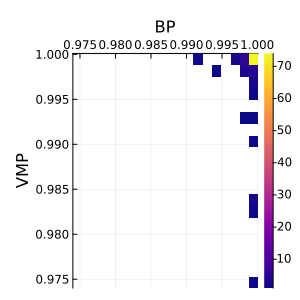
\includegraphics[width=1\linewidth]{uniform_dirichlet_percs_std125_t15.png}
  \caption{ $T = 15, N = 100$ }
  \label{fig:sub1}
\end{subfigure}%
\begin{subfigure}{.5\textwidth}
  \centering
  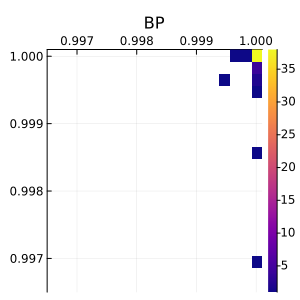
\includegraphics[width=1\linewidth]{uniform_dirichlet_percs_std125_t20.png}
  \caption{$T = 20, N = 50$}
  \label{fig:sub2}
\end{subfigure}
\caption{VMP ja BP algortimide protsentiilide kahedimensionaalne histogramm $N$ erineva katse mudeli \eqref{eq:hmm1}, \eqref{eq:hmm2}, \eqref{eq:hmm3} korral. Graafikute teljed pole võrdsed.}
\label{fig:test}
\end{figure}

\begin{table}[!htb]
    \caption{Esimeses kolmes reas kujutame leitud radade tõenäosusi protsentiilidena ning viimases neljas radade Hammingu kauguseid optimumist.}
    \begin{subtable}{.5\linewidth}
      \centering
        \caption{$T = 15, N = 100$}
        \begin{tabular} {l|l l l l l}
\toprule
{} & {mean} & {min} & {max} \\ 
\midrule
\text{BP} & 0.9995 & 0.9919 & 1.0 \\
\text{VMP} & 0.9986 & 0.9746 & 1.0 \\
\text{ORIG} & 0.8851 & 0.09 & 0.9999 \\
\\
\text{H vmp} & 1.63 & 0.0 & 7.0 \\
\text{H bp} & 1.61 & 0.0 & 7.0 \\
\text{H orgin} & 5.22 & 1.0 & 12.0 \\
\text{H naive} & 2.68 & 0.0 & 8.0 \\
\bottomrule
\end{tabular}
    \end{subtable}%
    \begin{subtable}{.5\linewidth}
      \centering
        \caption{$T = 20, N = 50$}
        \begin{tabular}{l|l l l l l}
\toprule
{} & {mean} & {min} & {max} \\ 
\midrule
\text{BP} & 0.99997 & 0.99955 & 1.0 \\
\text{VMP} & 0.99986 & 0.99701 & 1.0 \\
\text{ORIG} & 0.92382 & 0.48647 & 0.9998 \\
\\
\text{H vmp} & 2.1 & 0.0 & 7.0 \\
\text{H bp} & 1.74 & 0.0 & 5.0 \\
\text{H orig} & 6.96 & 3.0 & 14.0 \\
\text{H naive} & 3.06 & 0.0 & 8.0 \\
\bottomrule
\end{tabular}
    \end{subtable} 
\end{table}

\subsection{Vahelduva režiimiga mudel}\label{sec:switching_regime}

Vaatleme vahelduva režiimiga mudelit, mida loetakse müraga. Saame seda kirjeldada kolmekordse Markovi mudeli abil. Režiimi kirjeldagu Markovi ahel $\{U_t\}$, mille üleminekumaatriks olgu küllalt lähedal ühikmaatriksile ehk iga ajasammuga samma režiimi jäämine on suure tõenäosusega sündmus. On loomulik nõuda, et kõik režiimisisesed üleminekumaatriksid $P_u, u \in \{1,\ldots,U\}$ ei ole teineteisele lähedal KL kauguse mõttes. Kui igas režiimis on Markovi ahel sama, siis muutub režiimi ennustamine võimatuks. Igas režiimis $u \in \{1,\ldots,U\}$ kirjeldagu meid huvitavaid suurusi $x \in \{1,\ldots,X\}$ Markovi ahel $\{X_t\}$ $X \times X$ üleminekumaatriksiga $P_u$. Üleminekumaatrikseid iga $u$ ja $\Tilde{u} \ne u$ korral kirjeldagu maatriksid $P_u, P_{u \Tilde{u}}$, mis on saadud Dirichlet' jaotusest. Kirjutame kahekaupa Markovi mudeli üleminekumaatriksi kui $UX \times UX$ maatriksi
$$p =\begin{pmatrix} 
r_{11} P_1 & r_{12}P_{12} & \dots & r_{1u}P_{1u} \\
r_{21}P_{21} & r_{22}P_2 & \ldots & \vdots \\
\vdots & \dots & \ddots & \vdots \\
r_{u1}P_{u1} & \dots & \dots & r_{UU}P_{UU} 
\end{pmatrix}.$$

Keskendume järgmisena mõõtmisviisidele, mille abil kirjeldada kolmekordset Markovi ahelat genereerivaid mudeleid. Lühikeste realisatsioonide, nt $T \in \{ 10, 15, 20 \}$, korral me saame välja arvutada vastastikuse informatsiooni, mis ei ole praktikas realistlik.

Kirjeldamaks, milline on fikseeritud vaatlusandmete korral mittehomogeenne paarikaupa Markovi ahel, vaatleme järgnevaid entroopiaid ja KL kaugusi:
\begin{align*}
    \Delta_1 &:= \frac{1}{T}\sum_{t=1}^TD[p_{t} \| p_{u,t} \times p_{xt}]\\
    \Delta_2 &:= \sum_{t=2}^T D[p_{t-1,t} \| p_{t} \times p_{t-1}]\\
    \Delta_3 &:= D[p\| p_{1} \otimes \ldots \otimes p_{T}]\\
    \Delta_4 &:= H[q_u] + H[q_x]\\
    \Delta_5 &:= \sum_{t=1}^T H[q_t],
\end{align*}
kus $p_t$ on $(U_t,X_t)$ marginaali $\sum_{\bm{u}_{\setminus t}, \bm{x}_{\setminus t}} = p(\bm{u},\bm{x})$ jaotus ja $p_{u,t}(u_t) = \sum_{x_t}p_t(u_t,x_t)$.

Me kasutame KL kauguste aritmeetilist keskmist $\Delta_1$ mõõtmaks, kui lähedal on kahekordse mittehomogeense Markovi ahela jaotus $p$ jaotusele, mis sobib BP algoritmi rakendamiseks hästi, suurused $\Delta_2, \Delta_3$ näitavad, kui lähedal on jaotus $p$ jaotusele, mis sobib VMP rakendamiseks hästi. Entroopiaid $\Delta_4, \Delta_5$ kasutame hindamaks, kui enesekindlad me võime olla selles, et Viterbi rada on leitud - maksimaalse entroopiaga jaotused annavad samuti BP ja VMP algoritmide tulemustena mingid Viterbi raja hinnangud, aga nende puhul on Viterbi raja tõenäosus väike.

\subsubsection{Eksperimendid väikese $T$ korral}

Vaatleme $T \in \{10,20\}$ korral vastavalt $N = 100$ ja $N=50$ erinevat vahelduva režiimiga mudelit, kus me nõuame, et režiimisiseste üleminekumaatriksite $p_1,p_2,_3$ omavahelised KL kaugused oleksid suuremad kui $0.25$.

Me sobitame 

\begin{table}[!htb]
    \caption{\bla}
    \begin{subtable}{.5\linewidth}
      \centering
        \caption{$T = 10, N = 100$}
        \begin{tabular} {l|l l l l l}
\toprule
{} & {mean} & {min} & {max} \\ 
\midrule
\text{BP} & 0.9319 & 0.0586 & 1.0 \\
\text{VMP} & 0.9132 & 0.0264 & 1.0 \\
\text{ORIG} & 0.8416 & 0.0957 & 1.0 \\
\text{H vmp} & 2.24 & 0.0 & 9.0 \\
\text{H bp} & 2.32 & 0.0 & 10.0 \\
\text{H orig} & 3.07 & 0.0 & 8.0 \\
\text{H naive} & 2.47 & 0.0 & 6.0 \\
$\Delta_1$ & 0.0891 & 0.0143 & 0.2995 \\
$\Delta_2$ & 6.652 & 3.563 & 9.005 \\
$\Delta_3$ & 38.96 & 4.862 & 2347.0 \\
$\Delta_4$ & 4.569 & 0.76 & 7.803 \\
$\Delta_5$ & 10.78 & 4.179 & 19.65 \\
\bottomrule
\end{tabular}
    \end{subtable}%
    \begin{subtable}{.5\linewidth}
      \centering
        \caption{$T = , N = $}
        \begin{tabular}{l|l l l l l}
\toprule
{} & {mean} & {min} & {max} \\ 
\midrule
\text{BP} & 0.9319 & 0.0586 & 1.0 \\
\text{VMP} & 0.9132 & 0.0264 & 1.0 \\
\text{ORIG} & 0.8416 & 0.0957 & 1.0 \\
\text{H vmp} & 2.24 & 0.0 & 9.0 \\
\text{H bp} & 2.32 & 0.0 & 10.0 \\
\text{H orig} & 3.07 & 0.0 & 8.0 \\
\text{H naive} & 2.47 & 0.0 & 6.0 \\
$\Delta_1$ & 0.0891 & 0.0143 & 0.2995 \\
$\Delta_2$ & 6.652 & 3.563 & 9.005 \\
$\Delta_3$ & 38.96 & 4.862 & 2347.0 \\
$\Delta_4$ & 4.569 & 0.76 & 7.803 \\
$\Delta_5$ & 10.78 & 4.179 & 19.65 \\
\bottomrule
\end{tabular}
    \end{subtable} 
\end{table}